\documentclass{oci}
\usepackage[utf8]{inputenc}
\usepackage{lipsum}

\title{Suma de ejemplo}

\begin{document}
\begin{problemDescription}
  Finalmente ha llegado el día que todos estaban esperando:
  la fase final de la Olimpiada de Cachipún Interregional (OCI).
  En esta competencia, $n$ oponentes se enfrentan en $k$ rondas
  en la modalidad \emph{todos contra todos}.
  En cada ronda, los participantes deben elegir entre jugar piedra, papel o tijera.
  Como es tradicional, la tijera le gana al papel, el papel a la piedra y la piedra a
  la tijera.
  Luego de que todos los participantes revelan su opción de forma simultánea, se
  calcula el puntaje de acuerdo a la cantidad de victorias y derrotas.
  Específicamente, cada participante gana $1$ punto por cada victoria
  y pierde $1$ punto por cada derrota.
  Los empates no afectan la puntuación.

  Por ejemplo, considera una ronda para una competencia con $5$ participantes donde
  cada uno juega de la siguiente forma:
  \begin{center}
    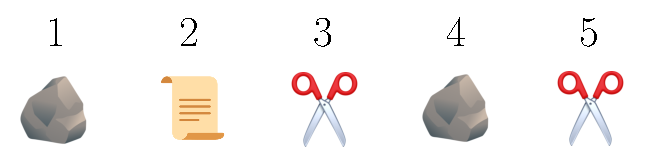
\includegraphics[scale=0.8]{ronda.eps}
  \end{center}
  Si nos concentramos en el participante 1, este le gana a los participantes 3 y 5
  (la piedra le gana al papel), sumando $2$ puntos.
  Adicionalmente, pierde contra el participante 2 (la piedra pierde contra el papel)
  lo cual resta $1$ punto.
  Finalmente, empata contra el participante 4 lo que no afecta el puntaje.
  Por consiguiente, el participante 1 obtiene puntaje igual a $1$ al final de la ronda.

  El \emph{puntaje final} de un participante luego de jugadas la $k$ rondas
  es igual a la suma de los puntajes que obtuvo en cada ronda.

  Históricamente, el registro de puntuación se ha manejado utilizando el
  Cachipún Management System (CMS), sin embargo, la organización ha encontrado
  una vulnerabilidad en el software, que parece ser muy difícil de arreglar.
  Es por esto que han decidió pedirte a ti que crees un nuevo programa que lo
  sustituya.

  Quedan menos de 4 horas para que comience la competencia, ¿podrás salvar la OCI?
\end{problemDescription}

\begin{inputDescription}
  La primera línea de la entrada contiene dos enteros $n$ ($2 \leq n \leq 1000$)
  y $k$ ($1 \leq k \leq 1000$), correspondientes a la cantidad de jugadores y de
  rondas respectivamente.
  Cada jugador es identificado con un entero entre 1 y $n$, mientras que las rondas
  con un entero entre 1 y $k$.

  Posteriormente, cada una de las siguientes $k$ líneas contiene $n$ enteros describiendo
  una ronda.  Específicamente, el $j$-ésimo entero de la $i$-ésima fila contiene la jugada
  del participante $j$ en la ronda $i$.
  Un $0$ representa que el participante jugó piedra, un $1$ que jugó un papel y un $2$
  que jugó tijera.
\end{inputDescription}

\begin{outputDescription}
  La salida debe contener $n$ enteros, donde el $i$-ésimo entero corresponde al
  puntaje final del jugador $i$.
\end{outputDescription}

\begin{scoreDescription}
  \subtask{20} Se probarán varios casos de prueba donde $n = 2$, es decir, hay exactamente $2$ jugadores.
  \subtask{40} Se probarán varios casos de prueba donde $n \leq 100$.
  \subtask{40} Se probarán varios casos de prueba sin restricciones adicionales.
\end{scoreDescription}

\begin{sampleDescription}
\sampleIO{sample-1}
\sampleIO{sample-2}
\sampleIO{sample-3}
\end{sampleDescription}

\end{document}
